\graphicspath{{chapters/method/figures/}}

\subsection{dummy_subsection_a}

\begin{frame}
  \frametitle{Qualitative results}
  \framesubtitle{Super-pixel classification vs Area-Overlap}
  \begin{figure}[Htbp]
    \centering
    \hspace*{\fill}%
      \subfigure[][Original Image, Ground Truth and Super-Pixels delineation.]{%
      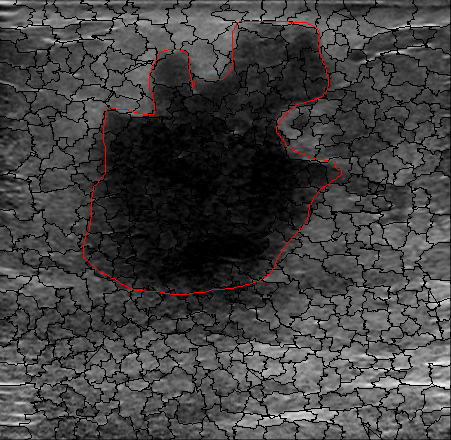
\includegraphics[width=.45\textwidth]{qualitativeResults/goodQSorigin}}
      \label{fig:dataTermb}%
      \hfill%
      \subfigure[][$\{\text{lesion}, \overline{\text{lesion}}\}$ labeling results, GT and SP delineation.]{%
      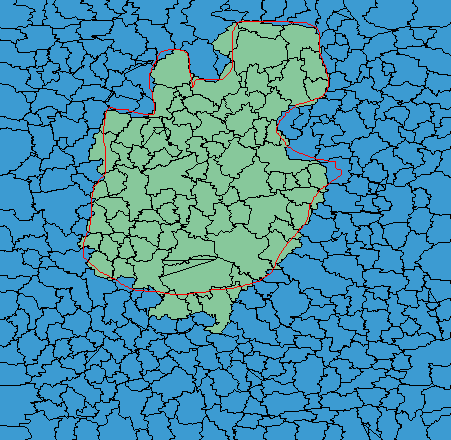
\includegraphics[width=.45\textwidth]{qualitativeResults/goodQSseg}}

      \label{fig:dataTermc}%
      \hspace*{\fill}%
        \label{fig:dataTerm}%
  \end{figure}
\end{frame}

\begin{frame}\frametitle{Qualitative results}
\framesubtitle{\footnotesize Influence of the Smoothing Term to False Positive Ratio}
\vspace{-10pt}
\begin{figure}[Htbp]
\setlength{\abovecaptionskip}{2pt}
\centering
\begin{tikzpicture}%[node distance=2cm]
  %       \node (a) {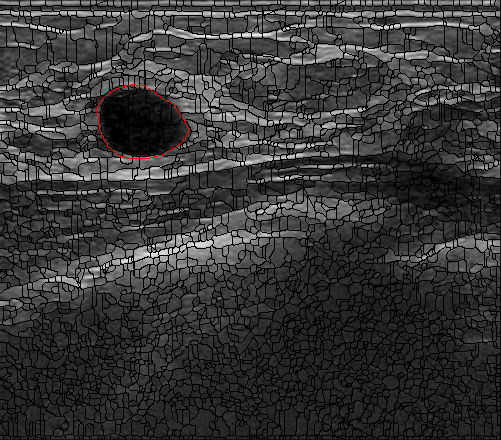
\includegraphics[width=.45\textwidth]{qualitativeResults/fporigin}};
  %%       \node [block, below of=a] (b) {B};
  %       \node [anchor=south west] (c) at ({.5\textwidth},0) {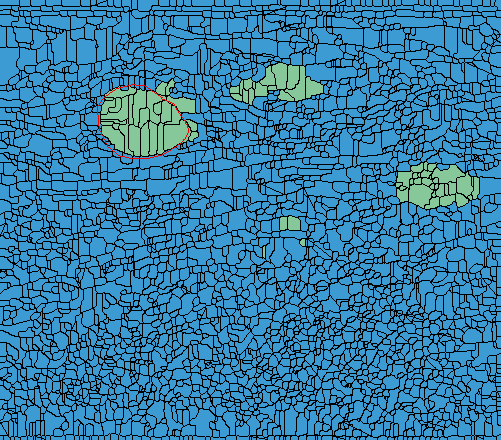
\includegraphics[width=.2\textwidth]{qualitativeResults/fpHom}};
  %       \node [anchor=north east] (d) at (a.north -| c.east) {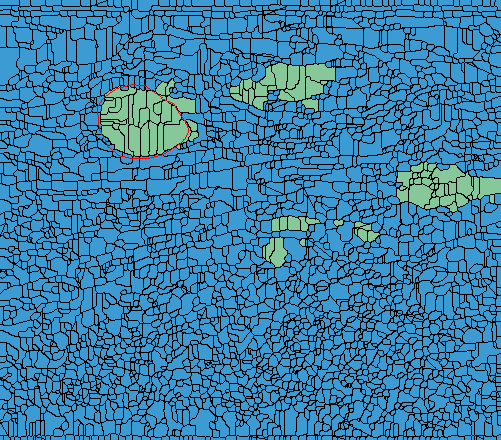
\includegraphics[width=.2\textwidth]{qualitativeResults/fpnohom}};
  %       
  \node [anchor=south west] (a) {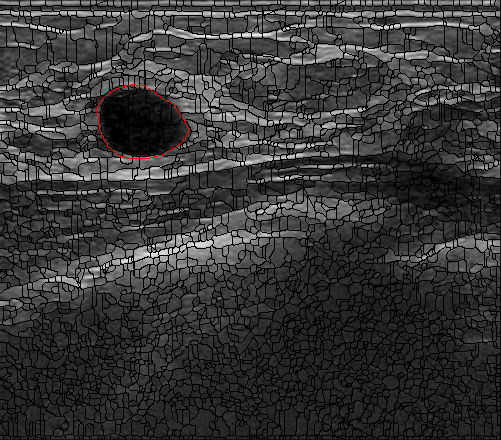
\includegraphics[height=.67\textheight]{qualitativeResults/fporigin}};
  \node [anchor =south west] (c) at ({.682\textwidth},0) {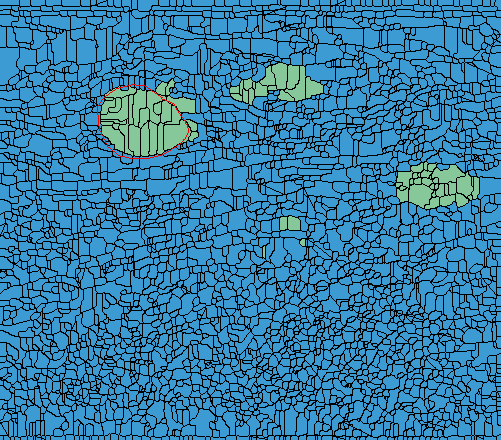
\includegraphics[height=.33\textheight]{qualitativeResults/fpHom}};
  \node [anchor = north west] (d) at (a.north -| c.west) {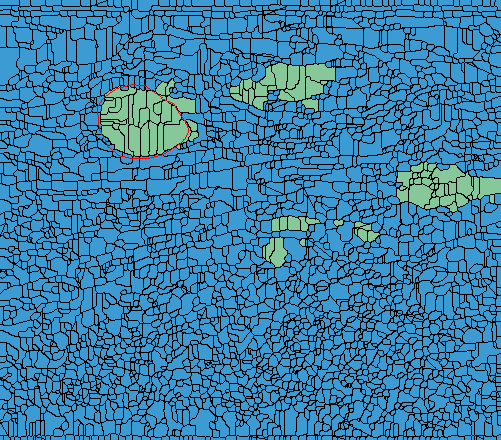
\includegraphics[height=.33\textheight]{qualitativeResults/fpnohom}};
\end{tikzpicture}

\end{figure}
\end{frame}

\subsection{dummy_subsection_b}
\begin{frame}[plain]\frametitle{Qualitative results}
\framesubtitle{When False Negative Emerge}
\vspace{-5pt}
\begin{figure}[Htbp]
\setlength{\abovecaptionskip}{2pt}
\centering
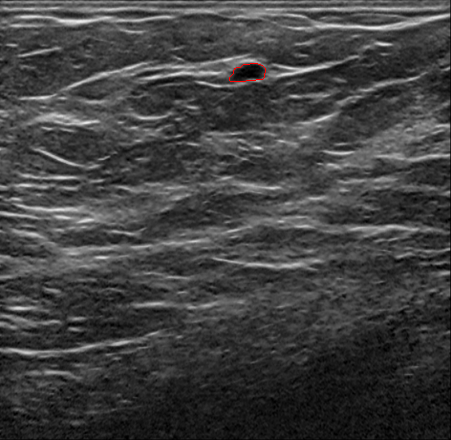
\includegraphics[width=.32\textwidth]{qualitativeResults/FNGT}~ 
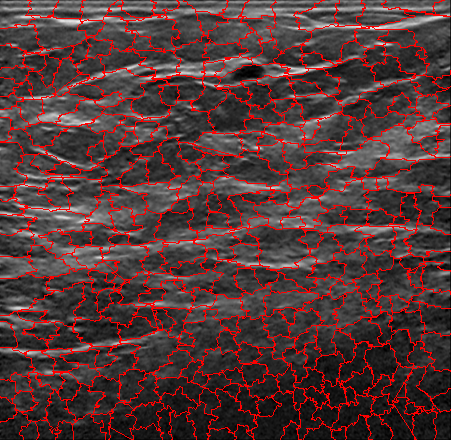
\includegraphics[width=.32\textwidth]{qualitativeResults/FNsp}\\ \vspace{3pt}
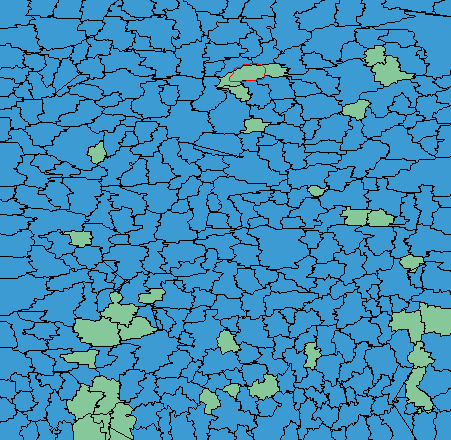
\includegraphics[width=.32\textwidth]{qualitativeResults/FNdetected}~ 
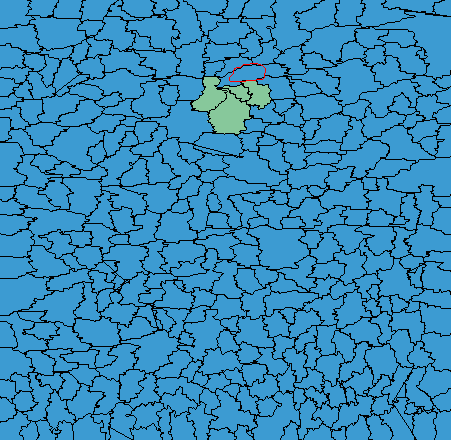
\includegraphics[width=.32\textwidth]{qualitativeResults/FNmiss}
\end{figure}
\end{frame}


\begin{frame}[plain]\frametitle{Quantitative Results}
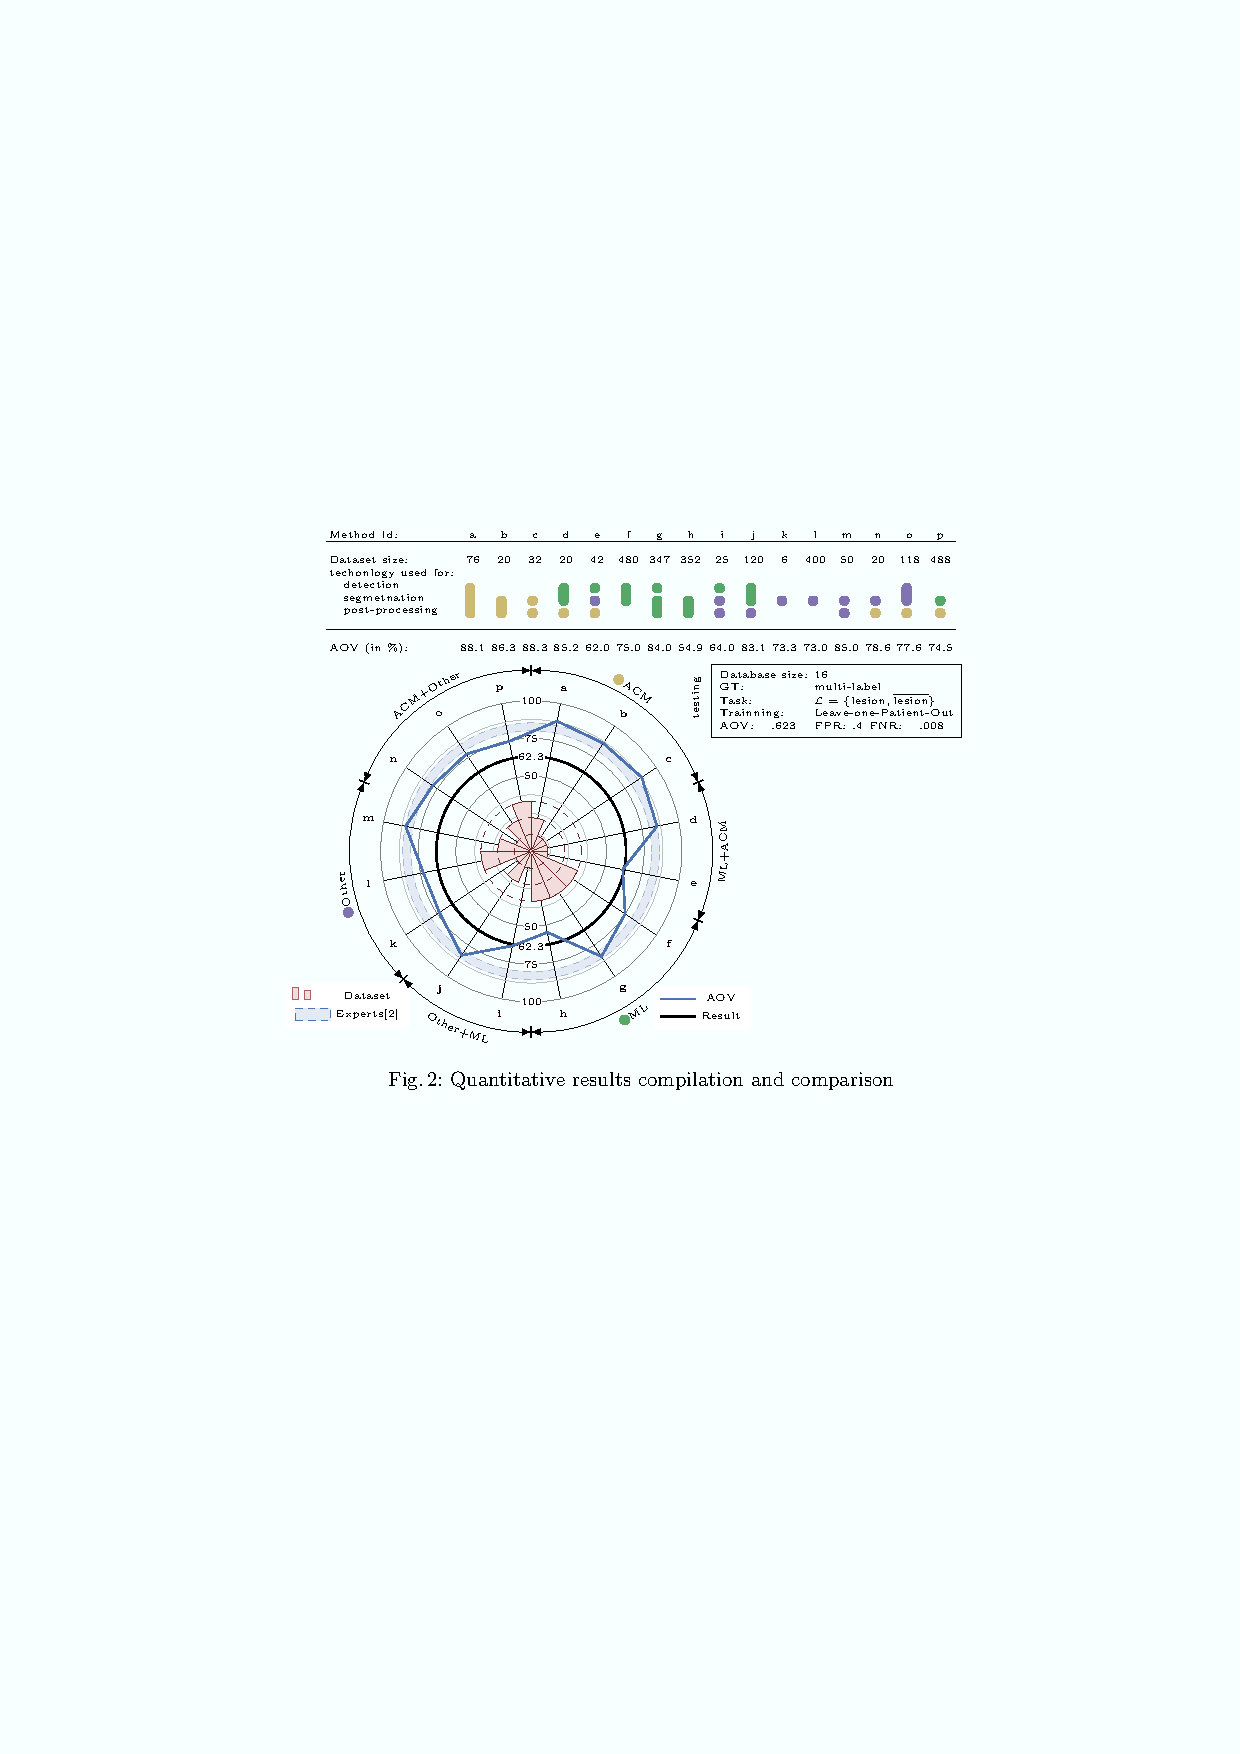
\includegraphics[trim=100 340 100 250,clip, height=.7\textheight]{quant.pdf} 
\end{frame}
